\documentclass[aspectratio=169,handout]{beamer}
\usepackage{borelian}

\begin{document}
    \classtitle{3}{Estadística descriptiva}{6 de enero de 2026}

    \begin{frame}{Motivación}
        La estadística nos ayuda con las siguientes tareas:

        \begin{itemize}
            \item Describir el comportamiento de fenómenos complejos utilizando conceptos sencillos (p. ej., el promedio).
            \pause
            \item Capturar aspectos esenciales de los datos como su estructura y saber qué tan incierto es el comportamiento generado en éstos.
            \pause
            \item Tomar decisiones mediante el análisis de datos, identificando tendencias y variabilidad en éstos.
            \pause
            \item Predecir resultados futuros a partir de datos pasados, sirviendo como base para modelos de aprendizaje automático.
        \end{itemize}

        \pause
        En inteligencia artificial, los datos y su tratamiento son una parte fundamental para construir modelos precisos. La estadística entrega herramientas y métodos para analizar y generar conocimiento sobre estos datos. 
    \end{frame}

    \begin{frame}{Ejemplo: grasas saturadas y carbohidratos}
        En el estudio ``PURE'', realizado con $\approx 135.000$ personas, se evaluó el riesgo de muerte por cualquier causa según el consumo de carbohidratos y grasas saturadas.
        \pause
        \begin{columns}
            \begin{column}{0.35\linewidth}
                \begin{figure}[H]
                    \centering
                    \includegraphics[width=\linewidth]{days/02/images/pure.png}
                \end{figure}
            \end{column}
            \hspace{-3mm}
            \begin{column}{0.6\linewidth}
                \begin{itemize}
                    \item Los resultados muestran que un mayor consumo de carbohidratos está ligado a una mayor tasa de muerte.
                    \pause
                    \item Lo inverso ocurre para las grasas saturadas.
                \end{itemize}
                Considerando el gráfico, ¿podemos asegurar que el consumo de grasas saturadas reduce la tasa de muerte?

                No, porque la existencia de correlaciones no implica que haya causalidad.
            \end{column}
        \end{columns}
    \end{frame}

    \begin{frame}{Un resumen de los principios de la estadística}
        La estadística se basa en los siguientes principios.
        \begin{itemize}
            \item \textbf{Aprendizaje de los datos}. La estadística es un conjunto de herramientas para postular hipótesis sobre los datos.
            \pause
            \item \textbf{Agregación}. En estadística, resumimos un conjunto de datos completo calculando valores que los describen.
            \pause
            \item \textbf{Incertidumbre}. En el mundo estadístico existen variables exógenas que no podemos medir o controlar.
            \pause
            \item \textbf{Muestreo}. Queremos sacar conclusiones sobre una población sacando datos de una muestra.
            \pause
            \item \textbf{Correlación y causalidad}. La correlación entre dos variables no implica causalidad.
        \end{itemize}
    \end{frame}

    \begin{frame}{¿Cómo aprendemos de los datos?}
        El análisis exploratorio de datos (en inglés, abreviado EDA) es un conjunto de técnicas que ayudan a entender los datos que se están trabajando.
        \begin{itemize}
            \item El objetivo central es intentar encontrar patrones en los datos que nos permitan postular hipótesis sobre ellos y/o el proyecto que contextualiza su análisis (p. ej., evaluación de factibilidad).
            \pause
            \item Puede ser dividido en descripción (cálculos estadísticos) y visualización de los datos. 
        \end{itemize}
        \pause
        En esta clase, hablaremos sobre estadística descriptiva. Mañana ahondaremos en la visualización de información.
    \end{frame}

    \begin{frame}[fragile]{Medidas de tendencia central: media}
        Las medidas de tendencia central intentan resumir datos de un conjunto en un valor único. La primera que veremos es la media o promedio. Dado un conjunto de datos $X = \{x_1, x_2, \dots ,x_n\}$, ésta se calcula como:
        \[ 
            \bar{X} = \frac{1}{n} \sum^n_{i=1} x_i  
        \]
        \pause
        El problema del promedio es que es muy sensitivo a \emph{outliers} (valores atípicos).
        \pause
        \begin{minted}{python}
            >>> import numpy as np
            >>> sample = [1, 2, 3, 100]
            >>> np.mean(sample)
        \end{minted}
    \end{frame}

    \begin{frame}{Hay que tener cuidado con los valores atípicos (\emph{outliers})}
        Los \emph{outliers} son valores atípicos en un conjunto de datos. Éstos valores se encuentran alejados de la distribución de los datos, y se pueden presentar en una variable o en interacciones entre varias variables.
        \pause
        \begin{columns}
            \column{0.5\linewidth}
            \begin{figure}[H]
                \centering
                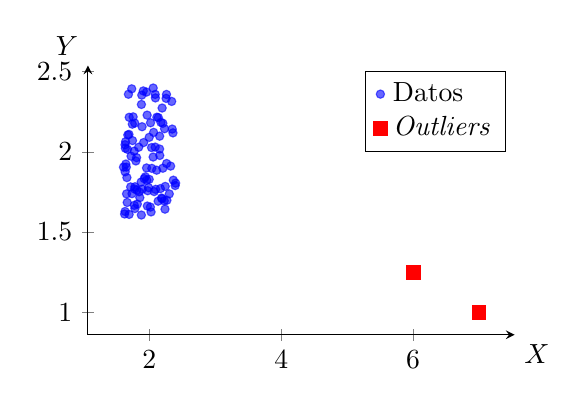
\begin{tikzpicture}
                    \begin{axis}[
                        axis lines=left,
                        width=7cm,
                        height=5cm,
                        xlabel={$X$},
                        ylabel={$Y$},
                        xlabel style={
                            at={(axis description cs:1,0)},
                            anchor=north west
                        },
                        ylabel style={
                            at={(axis description cs:0,1)}, 
                            anchor=south east,
                            rotate=-90
                        },
                        enlargelimits=0.1,
                        legend cell align=left,
                    ]
                        \pgfmathsetseed{42}
                        \addplot[
                            only marks, 
                            mark=*, 
                            blue, 
                            mark size=1.5pt, 
                            opacity=0.6,
                            samples=100, 
                            domain=0:1
                        ](
                            {2 + 0.4*rand},
                            {2 + 0.4*rand}
                        );
                        \addlegendentry{Datos}

                        \addplot[only marks, mark=square*, red, mark size=2.5pt] coordinates { 
                            (6,1.25) (7,1) 
                        };
                        \addlegendentry{\emph{Outliers}}
                    \end{axis}
                \end{tikzpicture}
            \end{figure}
            
            \column{0.5\linewidth}
            \pause
            \begin{itemize}
                \item Pueden deberse a errores de medición.
                \item Pueden representar eventos reales pero poco frecuentes.
                \item No deben ser eliminados ni imputados sin un previo análisis de por qué están presentes.
                \item Tienen un fuerte impacto en medidas como la media.
            \end{itemize}
        \end{columns}
    \end{frame}

    \begin{frame}[fragile]{Medidas de tendencia central: mediana}
        La mediana es el valor en la posición central de un conjunto de datos ordenado de menor a mayor. Para un conjunto de datos \textbf{ordenado} $X =\{x_1, x_2, \dots, x_n\}$, se calcula como:
        \begin{equation*}
            \textsf{mediana}(X) = \begin{cases} 
                x_{(n+1)/2} & \text{si $n$ es impar} \\
                \frac{x_{n/2} + x_{n/2+1}}{2} & \text{si $n$ es par} 
            \end{cases}
        \end{equation*}
        \pause
        En simple, es la observación que separa el conjunto de datos en una mitad de valores menores que él y otra mitad de valores mayores a él. 
        \pause
        \begin{minted}{python}
            >>> import numpy as np
            >>> sample = [1, 2, 33, 100, 4]
            >>> np.median(sample)
        \end{minted}
    \end{frame}

    \begin{frame}[fragile]{Medidas de tendencia central: moda}
        La moda es el valor que aparece con mayor frecuencia en un conjunto de datos. Para un conjunto de datos $X =\{x_1, x_2, \dots, x_n\}$, se define como:
        \[
            \textsf{moda}(X) = \underset{x_i \in X}{\arg\max} \; f(x_i)
        \]
        donde $f(x_i)$ es la frecuencia de aparición del valor $x_i$ en el conjunto $X$.
        \pause
        \begin{minted}{python}
            >>> from scipy import stats
            >>> sample = [1, 2, 2, 3, 4]
            >>> stats.mode(sample)
        \end{minted}
    \end{frame}

    \begin{frame}{Medidas de tendencia central: moda}
        La moda es especialmente útil para datos categóricos, donde la media y la mediana no son aplicables. Por ejemplo, en un conjunto de datos que representa colores favoritos, la moda sería el color que más personas prefieren.
        \pause
        \begin{itemize}
            \item Un conjunto de datos puede tener más de una moda (bimodal, multimodal).
            \pause
            \item La moda es menos sensible a valores atípicos en comparación con la media. ¿Se les ocurre por qué?
        \end{itemize}
        \pause
        \begin{exampleblock}{Ejemplo}
            \begin{columns}
                \begin{column}{0.6\linewidth}
                    Consideremos el conjunto de datos simplificado que muestra las edades y alturas de tres personas.

                    ¿Cuál es la moda de las alturas? ¿Por qué? ¿Y la moda de las edades?                    
                \end{column}
                \hfill
                \begin{column}{0.3\linewidth}
                    \begin{table}[H]
                        \centering
                        \begin{tabular}{c|c|c}
                            $X$ & Edad & Altura (\textrm{m}) \\ \hline
                            $x_1$ & $17$ & $1.76$ \\
                            $x_2$ & $29$ & $1.76$ \\
                            $x_3$ & $10$ & $1.58$                
                        \end{tabular}
                    \end{table}
                \end{column}
            \end{columns}
        \end{exampleblock}
    \end{frame}

    \begin{frame}{Comparación entre media, mediana y moda}
        Es interesante ver como cambian estas medidas de tendencia central según el tipo de distribución:
        \begin{figure}
            \centering
            \includegraphics[width=0.8\linewidth]{days/02/images/mean_mode_median.png}
        \end{figure}
    \end{frame}

    \begin{frame}[fragile]{Medidas de tendencia central (percentiles)}
        La mediana puede ser generalizada con el concepto de percentil. Los percentiles dividen los datos ordenados de menor a mayor en 100 partes iguales.
        \begin{itemize}
            \item El percentil 50 (denotado $P_{50}$) corresponde a la \textbf{mediana}.
            \pause
            \item Los percentiles 25 ($P_{25}$) y 75 ($P_{75}$) definen el \textbf{rango intercuartílico}. También son conocidos como cuartil 1 ($Q_1$) y cuartil 3 ($Q_3$) respectivamente.
            \pause
            \item $P_{25}, P_{50}$ y $P_{75}$ dividen la muestra en $4$ partes que son descritas mediante los \emph{boxplots}.
        \end{itemize}
        \pause
        \begin{columns}
            \column{0.5\linewidth}
            \begin{minted}{python}
                >>> import numpy as np
                >>> sample = [1, 2, 3, 4, 100]
                >>> np.percentile(sample, 25)
                >>> np.percentile(sample, 75)
            \end{minted}

            \column{0.5\linewidth}
            \pause
            \begin{figure}
                \centering
                \includegraphics[width=\linewidth]{days/02/images/boxplot.png}
            \end{figure}
        \end{columns}
    \end{frame}

    \begin{frame}{La interpretación estadística \textbf{SÍ} importa}
        Consideremos un caso típico de análisis estadístico. Tomemos una muestra con $5$ chilenos, cada uno representado por una entrada en $X = \{x_1, x_2, x_3, x_4, x_5\}$, y sus respectivos sueldos:
        \begin{table}[H]
            \centering
            \begin{tabular}{c|c}
                $X$ & Sueldo (CLP) \\ \hline
                $x_1$ & $\$\, 300\,000$ \\
                $x_2$ & $\$\, 10\, 000\,000$ \\
                $x_3$ & $\$\, 75\,000$ \\
                $x_4$ & $\$\, 510\,000$ \\
                $x_5$ & $\$\, 7\,500\,000$
            \end{tabular}
            \caption{Sueldo mensual de una muestra de personas chilenas.}
            \label{tab:chilean-earnings}
        \end{table}
        \vspace{-3mm}
        \pause
        \begin{itemize}
            \item ¿Cuál es el valor del promedio $\overline{X}$? ¿Y de $\textsf{mediana}(X)$?
            \pause
            \item ¿Qué pasa si sólo nos enfocamos en informar sobre el promedio?
        \end{itemize}
    \end{frame}

    \begin{frame}{Medidas de dispersión}
        \begin{columns}
            \begin{column}{0.45\linewidth}
                \justifying
                \begin{block}{Definición}
                    \justifying
                    Las medidas de dispersión se vinculan con estadísticos que permiten describir la variabilidad de los datos en una muestra con respecto a una medida de tendencia central (usualmente la media).
                \end{block}
                La figura \ref{fig:scatter-variability} muestra la dispersión en un conjunto de puntos. \textbf{¿Cómo la resumimos en un número real?}
            \end{column}
            \begin{column}{0.5\linewidth}
                \begin{figure}[H]
                    \centering
                    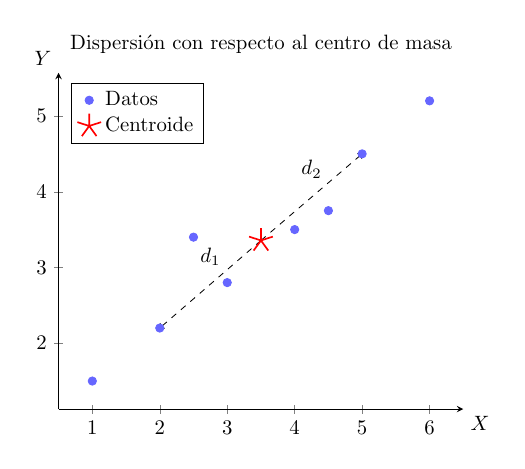
\begin{tikzpicture}[scale=0.75]
                        \def\dataset{1/1.5, 2/2.2, 3/2.8, 4/3.5, 5/4.5, 2.5/3.4, 4.5/3.75, 6/5.2}
                    
                        \def\sumx{0} 
                        \def\sumy{0} 
                        \def\countn{0}
                        \def\coords{}
                    
                        \foreach \x/\y in \dataset {
                            \pgfmathparse{\sumx+\x} \xdef\sumx{\pgfmathresult}
                            \pgfmathparse{\sumy+\y} \xdef\sumy{\pgfmathresult}
                            \pgfmathparse{\countn+1} \xdef\countn{\pgfmathresult}
                            
                            \xdef\coords{\coords (\x,\y)}
                        }
                    
                        \pgfmathsetmacro{\meanx}{\sumx/\countn}
                        \pgfmathsetmacro{\meany}{\sumy/\countn}
                    
                        \begin{axis}[
                            title={Dispersión con respecto al centro de masa},
                            axis lines=left,
                            xlabel={$X$},
                            ylabel={$Y$},
                            xlabel style={
                                at={(axis description cs:1,0)},
                                anchor=north west
                            },
                            ylabel style={
                                at={(axis description cs:0,1)}, 
                                anchor=south east,
                                rotate=-90
                            },
                            legend pos=north west,
                            legend cell align=left,
                            enlargelimits=0.1
                        ]
                            \addplot[only marks, mark=*, blue!60] coordinates {\coords};
                            \addlegendentry{Datos}
                            
                            \addplot[
                                only marks,
                                mark=star, 
                                mark size=6pt,
                                color=red,
                                thick
                            ] coordinates {(\meanx, \meany)};
                            \addlegendentry{Centroide}

                            \coordinate (centroid) at (\meanx, \meany);

                            \coordinate (point1) at (2, 2.2);
                            \coordinate (point2) at (5, 4.5);
                            
                            \draw[->,dashed] (centroid) -- node[above,yshift=2mm] {$d_1$} (point1);
                            \draw[->,dashed] (centroid) -- node[above,yshift=2mm] {$d_2$} (point2);
                        \end{axis}
                    \end{tikzpicture}
                    \caption{Dispersión de puntos en el espacio $\mathbb{R}^2$.}
                    \label{fig:scatter-variability}
                \end{figure}
            \end{column}
        \end{columns}
    \end{frame}

    \begin{frame}[fragile]{Medidas de dispersión: varianza}
        La varianza mide qué tan dispersos están los datos con respecto a la media aritmética. Para un conjunto $X = \{x_1, x_2, \dots, x_n\}$, se puede calcular como:
        \[ 
            \mathbb{V}\textsf{ar}(X) = \frac{1}{n-1} \sum^n_{i=1} \left(x_i - \bar{X}\right)^2 
        \]
        lo que es análogo a un promedio de distancias considerando $n-1$ grados de libertad.
        \pause
        \begin{minted}{python}
            >>> import numpy as np
            >>> sample = [8, 3, 5, 10]
            >>> np.var(sample, ddof=1) # ddof=1 permite dividir por n-1
        \end{minted}
        \pause
        \begin{block}{Pregunta}
            ¿Cuál es la varianza de la muestra $X = \{1, 1, \dots, 1\}$ (sólo unos)?
        \end{block}
    \end{frame}

    \begin{frame}[fragile]{Medidas de variabilidad: covarianza}
        Para cuantificar cuánto varia una variable con respecto a otra utilizamos metricas multivariadas. 

        \pause
        La covarianza $\textsf{cov}(X,Y)$ mide el grado de cambio lineal en conjunto de dos variables $X$ e $Y$, y se calcula como:
        \[ 
            \textsf{cov}(X,Y) = \frac{1}{n-1} \sum^n_{i=1} (x_i - \bar{X}) (y_i - \bar{Y}) \in (-\infty, +\infty)
        \]
        \pause
        Una covarianza positiva indica que ambas variables tienden a aumentar juntas, mientras que una covarianza negativa indica que una variable tiende a aumentar cuando la otra disminuye. Si es cero, no hay una relación lineal entre las variables, pero puede ser no lineal.
        
        \pause
        \begin{minted}{python}
            >>> import numpy as np
            >>> X = [42, 9, 21, 31]
            >>> Y = [3, 2, 1, 11]
            >>> print(np.cov(X,Y))
        \end{minted}
    \end{frame}

    \begin{frame}[fragile]{Medidas de variabilidad (covarianza y correlación)}
        \begin{itemize}
            \item Si dos variables $X$ e $Y$ son independientes, entonces su covarianza será $0$ (¡al revés esta afirmación no necesariamente es cierta!).
            \pause
            \item Si la dependencia entre $X$ e $Y$ se puede aproximar mediante una recta, entonces diremos que existe una \textbf{correlación lineal} entre ellas.
        \end{itemize}

        \pause
        Una métrica bastante importante es el coeficiente de correlación de Pearson $\rho(x,y)$, que estima la relación entre dos variables independiente de su magnitud, lo que permite que la interpretación sea más intuitiva:
        \[
            \rho(x,y) = \frac{cov(x,y)}{sd(x)sd(y)} \in [-1, 1]
        \]

        \pause
        Si es $1$, existe una correlación lineal positiva perfecta. Si es $-1$, existe una correlación lineal negativa perfecta. Si es $0$, no existe correlación lineal entre las variables.
        \end{frame}
\end{document}